%------------------------------------------------------------------------------
% This is a LaTeX template for the scientific justification of IRAM Proposals 
%------------------------------------------------------------------------------
% 
% We encourage IRAM proposers to use this template for the sake of unity 
% and clarity when Program Committee members assess their proposals.
% 
% You may customize this template to suit your preferences (e.g. using BibTex),
% but please respect the following requirements:
%     The scientific justification should contain a maximum of 2 pages of text 
%     (4 pages for Large Programs), plus 2 pages of Figs., Tables and Refs.
%     The font size should be 11pt or larger.
%
% For Large Programs, the following sections should be included: 
%   i) Scientific Rationale, 
%  ii) Immediate Objective, 
% iii) Feasibility and Technical Justification, and 
%  iv) Organizational Issues.
% 
%
%------------------------------------------------------------------------------
%
\documentclass[11pt,a4paper,twoside,graphicx,color]{article}
%
\usepackage[margin=2cm]{geometry}
\usepackage[pdftex]{graphicx}
\usepackage{color}
\usepackage{txfonts}
\usepackage{paralist}
\usepackage[numbers]{natbib}
\setlength{\bibsep}{0.0pt}
\usepackage{amssymb}

\newcommand{\ccor}[1]{\textcolor{red}{#1}}

\bibpunct{(}{)}{;}{a}{}{,} % to follow the A&A style
\bibliographystyle{aa} % style aa.bst

%
% Page size and text dimensions
% Do not change!
\textheight 260mm
\textwidth 178mm
\oddsidemargin -8mm
\evensidemargin -8mm
\marginparwidth 50pt
\topmargin -22mm
\brokenpenalty=10000
\sloppy
%
%-------------------------------------------------------------------
\begin{document}
%
%
\begin{center}{\huge \bf
%-------------------------------------------------------------------
High resolution observations of the thermal SZ effect on galaxy clusters
%-------------------------------------------------------------------
}\end{center}
% 
\begin{center}
J. F. Mac\'ias-P\'erez (LPSC), E. Pointecouteau (IRAP), B. Comis (LPSC), R. Adam (LPSC), N. Aghanim (IAS), M. Arnaud (CEA), F.X. D\'esert (IPAG), M. Douspis (IAS), F. Mayet (LPSC), P. Mauskopf, J. B. Melin (CEA), L. Perotto (LPSC), G. Pratt (CEA), J. A. Rubi\~no-Mart\'in (IAC), F. Ruppin (LPSC)
\end{center}

%-------------------------------------------------------------------
\vspace{-0.3cm}
%\section{Scientific context}
%\vspace{-0.3cm}
{\bf Abstract -- } 
We describe here the NIKA2 Guaranteed Time Large Program dedicated to high resolution observations of clusters of galaxies at intermediate and high redshift via the thermal Sunyaev-Zeldovich (tSZ) effect for a total of 300 hours. NIKA2 is well adapted for high angular resolution follow-up observations because of its large number of high sensitive detectors observing at two frequency bands (150 and 260 GHz), its large field of view (6.5 arcmin) and the resolution allowed by a 30 m telescope (17.5 and 11 arcsec, respectively at the two frequencies). We intend to observe a large ($\gtrsim$ 50) and cosmologically representative sample of clusters of galaxies, with redshift between 0.5 and 1.5, to which the f.o.v. and resolution of NIKA2 are better suited. The main output of the program will be the study of the redshift evolution of the cluster pressure profiles and of the scaling laws relating cluster observational parameters such as the integrated Compton parameter (Y) and the electron temperature (T$_e$), for example, to their total mass (M$_{tot}$). This can be achieved with through NIKA2 tSZ observations and by combining them with ancillary data, including X-rays and optical observations, leading to significant improvements on the use of clusters of galaxies to draw cosmological constraints.\\

\vspace{-0.1cm} \noindent {\bf \large Scientific context -- }
As the largest gravitationally collapsed objects, clusters of galaxies represent the last step of the hierarchical gravitational process of structure formation. Therefore their abundance and evolution are strictly related to the power spectrum of the primordial density fluctuations, cosmological parameters and their evolution all along the history of our Universe. 
Clusters are mainly made up of dark matter (85\%), while most of the baryons are present as a diffuse gas, the Intra-Cluster Medium (ICM), hot (10$^6$ - 10$^8$ K) and completely ionized because of the incredibly high masses characterizing this kind of structures (10$^{13}$ - 10$^{15}$ M$_{\odot}$). Since the ICM is a very good tracer of the dark matter distribution, ICM observables can provide a valuable tool for cosmological investigation with clusters, as long as we are able to convert them into mass estimates. From baryonic observables the total mass can be inferred through scaling relations, which correspond to power laws obtained in a simplified scenario in which gravity is the only process driving cluster evolution. At present, the systematic uncertainties affecting the observable to mass relations represent the limit for cluster-derived cosmological constraints. Therefore we need to improve our knowledge of the statistics of galaxy cluster structure in order to reduce the deriving uncertainties and bias for cosmological studies \citep[e.g.][]{number_counts2015, ymap}.

Due to its physical state, the ICM is responsible of a secondary anisotropy of the Cosmic Microwave Background (CMB), which is the thermal Sunyaev-Zel'dovich (SZ) effect. Through their path toward us, CMB photons interact with free hot electrons in the ICM. After this interaction a fraction of CMB photons is moved to higher energies, with a resulting flux decrement (increment) at frequencies below (above) 217 GHz. The amplitude of the deformation is proportional to the integral of the pressure of the electron population along the line of sight. While optical and X-ray cluster signals are affected by cosmological dimming, this is not the case for the tSZ cluster signal. Therefore the tSZ effect allows us to detect and study cluster of galaxies at high redshifts, where their number and distribution is the most sensitive to the underlying cosmology.
In the last few years, technological progress have made the tSZ effect routinely detected and SZ-selected cluster catalogues containing several hundreds of candidates have finally been produced, with arcmin resolution, by the South Pole Telescope \citep[SPT, FWHM $\sim$ 1.1 arcmin at 150 GHz,][]{Reichardt2013, Bleem2014}, the Atacama Cosmology Telescope \citep[ACT, FWHM $\sim$ 1.4 arcmin at 148 GHz, ][]{Hasselfield2013}, the Planck Satellite \citep[FWHM $\sim$ 10 arcmin for SZ,][]{PSZ1, PSZ2}.  Planck, ACT and SPT have detected many clusters through tSZ performing a blind survey able to use this effect to identify objects not yet discovered at other wavelengths. However their relatively limited resolutions ($\gtrsim$ 1 arcmin) only allow detailed study of the spatial distribution of the signal for low redshift clusters (z $<$ 0.2). But the use of tSZ-selected cluster samples for cosmological purposes requires the understanding the details of how matter (baryonic and dark) is distributed and the evaluation of the scatter that disturbed systems may introduce in the relation between the tSZ integrated flux (Y) and the cluster total mass (M$_{tot}$).Therefore, measurements reaching sub-arcminute angular resolution for cluster pressure profiles are a mandatory step for precise cluster cosmology. 

The NIKA camera at the IRAM 30~m telescope is a well-suited instrument for such observations and follow-ups, given its resolution, sensitivity and dual-band observation capability (as it will be detailed later). These in depth investigations over a large redshift range will bring detailed insight of the properties of clusters over more than 3 Gyr, allowing us to understand the processes driving the physical evolution of massive halos in the universe.


\vspace{0.3cm} \noindent {\bf \large Main scientific goals -- } 
Clusters grow by constant smooth accretion and violent merger events. This mechanism driving
the growth of structures impacts cluster content, and thereby this complex accretion history imprints
the energy distribution within the ICM. 
Furthermore, feedback from galaxy formation (through AGN and SFR/SN) also impacts the properties of the gas, injecting energy within the ICM which is known to counterbalance the gravitational radiative cooling of the hot gas. These energy injections modify the thermodynamical state of the ICM and then they might also affect its observable properties, in a way that must be quantified.

We have now a fairly good view of the ICM distribution in the local Universe, mainly at
redshift below 0.5. This has been possible because of recent tSZ measurements (e.g. \citealt{PPP, Plagge2010}) that are a
powerful diagnostic of the physical state of the hot intra-cluster gas. Indeed the tSZ effect is directly proportional to the
thermal pressure integrated along the line of sight. Then measuring the (radial) distribution of the SZ
signal in clusters directly probes the distribution of thermal pressure within the ICM. 
%By contrast X-ray measurements are sensitive to the square of the gas density and the root square of the temperature. 
%We present in Figure 1 recent measurements of the stacked cluster radial pressure profile using tSZ observations with PLANCK, BOLOCAM and SPT and X-ray estimates. From the
%left plot we can notice that the tSZ measurements are in good agreement but are not able to sample the inner part of the clusters, which present a cool-core (CC), and disturbed ones (non-CC). This is more obvious 

However, in order to investigate the details of the SZ cluster morphology up to high redshift, we must perform high angular resolution (sub-arcmin) SZ observations.
This will in fact allows us to investigate how cluster properties evolve with time, in order to understand the mechanisms ruling the formation and the evolution of structures.
The investigation of the physical state of groups and clusters as a function of redshift will thus help us to asses 
the evolution involved by the cluster accretion history, the processes at play in a gravitationally bound
system and spread light on the co-evolution of the different  cluster baryonic components (i.e. the hot intra-cluster gas and the cluster galaxies). 
Carrying such a study for the SZ observable over a population of high redshift
clusters will allow to quantify whether the thermal content and its distribution evolve as massive
halos continue to growth through accretion and merger. Such measurements will only be made possible by high sensitivity and high spatial resolution tSZ observations. 

The NIKA2 camera is particularly well adapted for high resolution observations of the tSZ effect on cluster of galaxies:
\begin{itemize}
\item [a)] It operates simultaneously at two frequency bands: 150 and 260 GHz (Figure \ref{Fig:bands}). As shown on the bottom panel of Figure \ref{Fig:bands}, we expect for 150 and 260 GHz, respectively, a negative and a positive distortion of the CMB spectrum producing a very distinctive cluster signal on the observed maps. 
\item [b)] NIKA2 is made of arrays of thousands of high sensitive Kinetic Inductance Detectors (KIDs). In particular we expect a sensitivity in Compton parameter units of 1.13 x10$^{-4}$ per hour and per beam. This should allow us to obtain reliable tSZ detections of clusters of galaxies in few hours.
\item [c)] NIKA2 coupled to the IRAM 30 m telescope allows us to map clusters of galaxies to a resolution of typically 12 to 20 arcsec within a 6.5 arcmin diameter FOV. This is well adapted for medium and high redshift clusters for which we expect typical angular sizes of about 6-11 arcmin (Figure \ref{Fig:size}).
\end{itemize}

NIKA2 SZ capabilities have been demonstrated through an SZ pilot study conducted with its pathfinder, NIKA. In the context of this pilot study we have mapped the SZ signal in the direction of six clusters of galaxies, validating the KIDs capabilities when dealing with such a faint and diffuse signal \citep[][dedicated to an intermediate redshift cluster, RX J1347.5-1145]{Adam2014}, even at very high redshift \citep[CL J1226.9+3332, at z~$=$~0.89,][]{Adam2015} and at the level of detection of the Planck catalogue of SZ sources (NIKA Collaboration in preparation).

With NIKA2 the cluster gas will be finally mapped in SZ with a quality (in terms of sensitivity and angular resolution) comparable to X-ray, even for intermediate and high-redshift clusters. Then, the natural combination of direct observables of the intra-cluster hot gas (i.e., SZ and X-ray measurements), as well as of the dark matter distribution (i.e, optical weak lensing measurements), will allow a full physical characterization of the (radial) distribution of the physical properties of clusters. %including pressure, entropy, gas mass, total mass, gas fraction and clumpiness of the gas. 
Indeed, the tSZ signal directly probes the gas pressure, while X-ray data deliver the gas density squared and temperature. The combination of the two observables is the only way to provided an unbiased estimate of the entropy and clumpiness of the gas: pressure profiles (P$_e$(r)) with spatial resolution comparable to those of X-ray derived electron densities (n$_e$(r)) can be used to study the cluster radial distribution of temperature  (T$_{e}$(r) $\propto$ P$_{e}$(r)/n$_{e}$(r)) and entropy (K(r) $\propto$ P$_{e}$(r)n$_{e}^{-5/3}$), which are essential to unveil cluster thermodynamic history.
In addition, weak lensing measurements will provide complementary measurements of the dark matter distribution and total mass of the clusters, in a totally independent way, then affected by different systematics.
Furthermore, the combination of the SZ and X-ray data to optical/NIR observations of the cluster galaxies will further help to investigate the connection between galaxy properties (luminosity function, SFR, stellar mass) and those of the ICM, and thereby bring constraints on feedback mechanisms at play within clusters.

\begin{figure}
  \begin{center}
   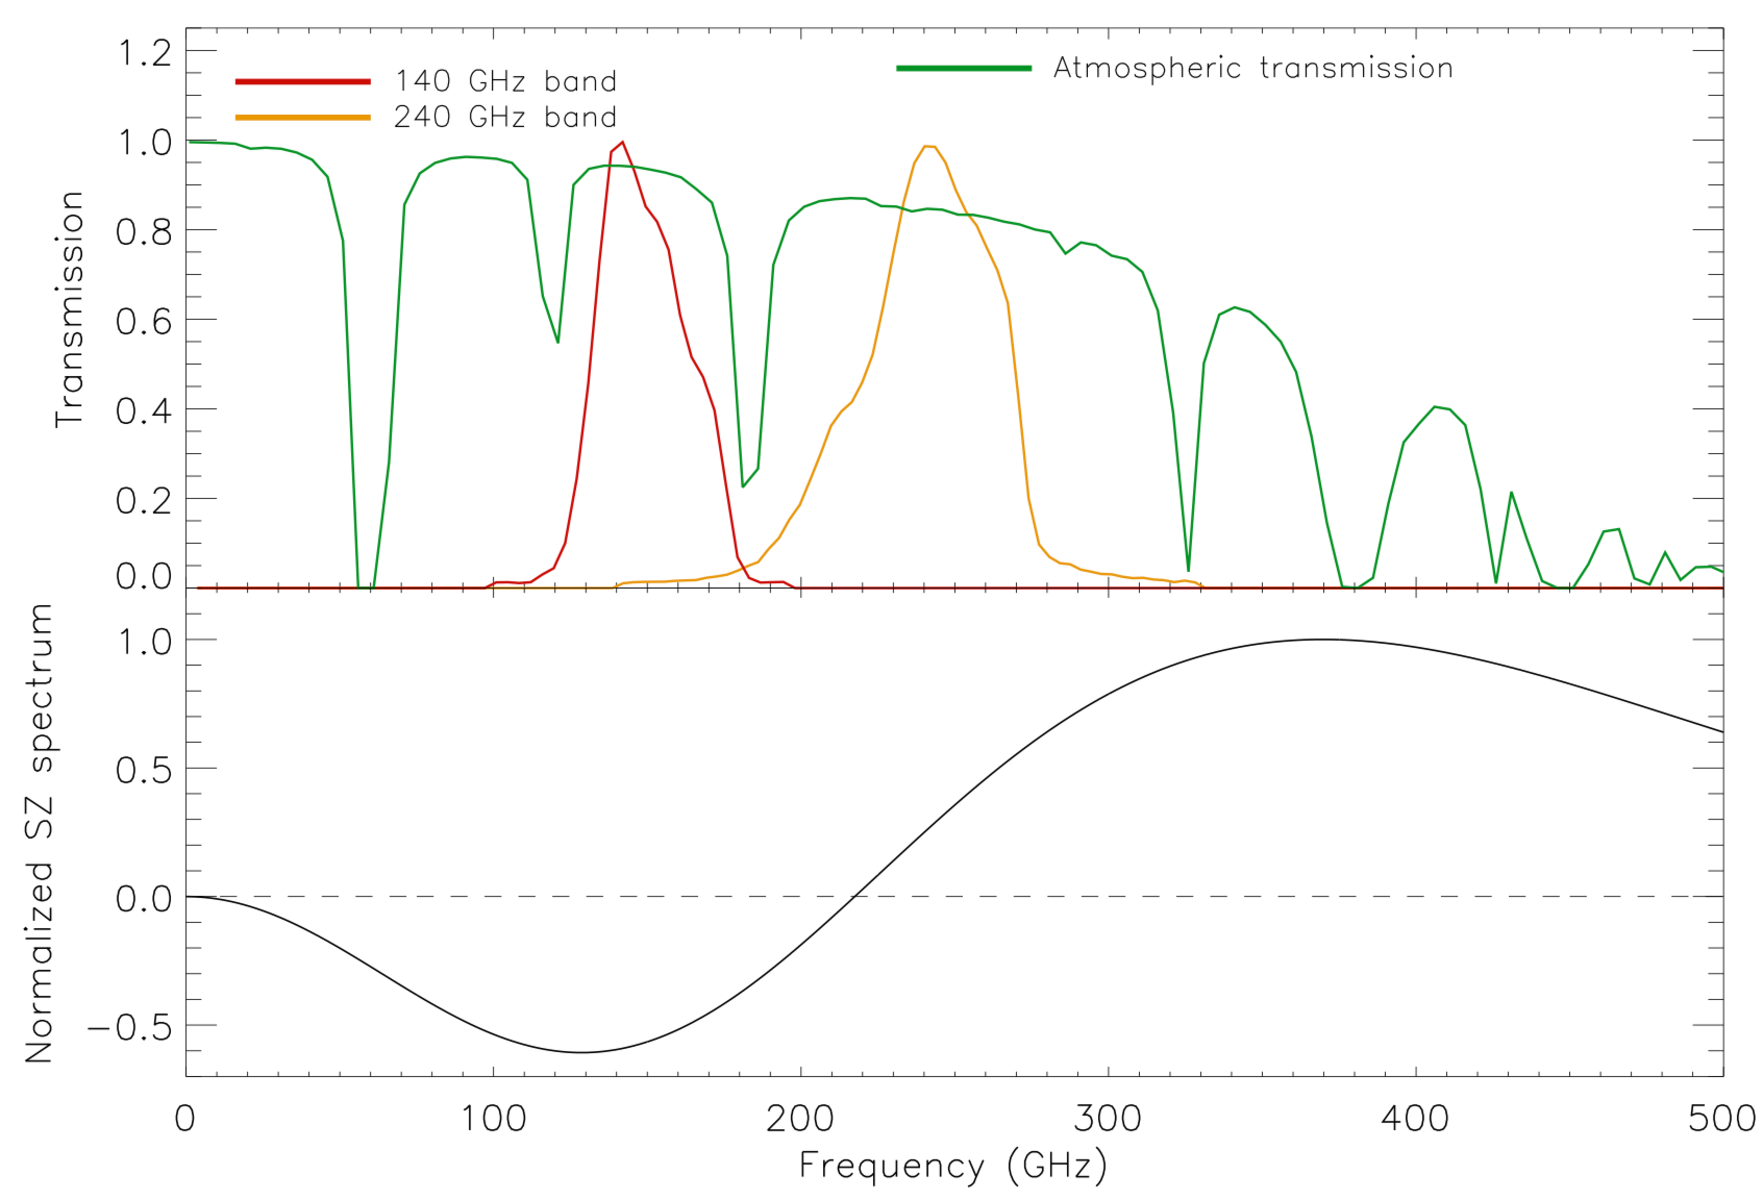
\includegraphics[width=0.6\columnwidth]{./Figures/NIKA_bp_sz.pdf}
  \end{center}
\caption{{\bf Top:} The bandpasses of the current NIKA KIDs arrays at 140 (red) and 240 (orange) GHz and the atmospheric transmission at Pico Veleta (Spain), the IRAM 30m telescope site. {\bf Bottom} The spectral distortion of the CMB intensity induced by the tSZ effect.}
\label{Fig:bands}
\end{figure}

\begin{figure}
  \begin{center}
   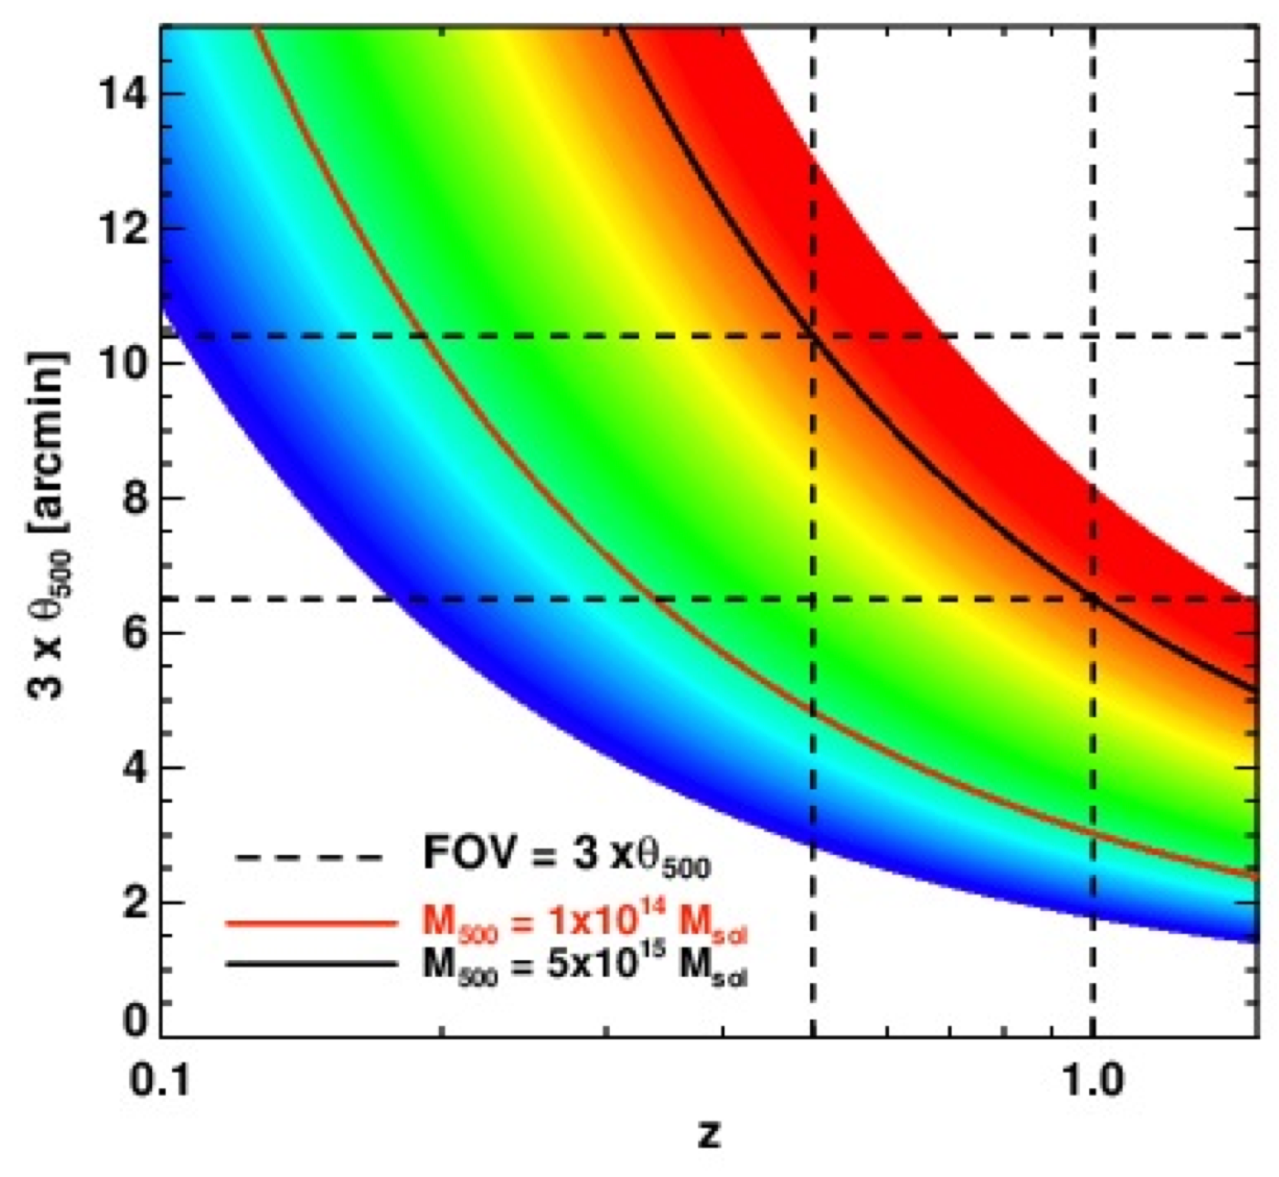
\includegraphics[width=0.6\columnwidth]{./Figures/size_vs_z.pdf}
  \end{center}
\caption{Evolution of the angular size (as 3x$\theta$500 for the field to be covered) with redshift according to a large range of masses. 10$^{14}$ and 5$\times$10$^{15}$ M$_{\odot}$ are shown as red black lines respectively. The dashed lines mark the field of view required to cover 3x$\theta$500 for a 5$\times$10$^{15}$ M$_{\odot}$ cluster within the redshift interval of interest (i.e., 0.5 $<$ z $<$ 1.0)}
\label{Fig:size}
\end{figure}

\vspace{0.3cm} \noindent {\bf \large Comparison with other high-angular resolution SZ facilities -- } 
It is important to compare NIKA2 to other existing and planned instruments for high resolution tSZ observations. 

Interferometers can reach extremely high angular resolutions (i.e. CARMA, ALMA), but they cannot recover the large scale signal and they are time expensive. Other experiences exist that operate at the focus of large diameter telescopes. However none of them can combine a sufficiently large f.o.v. with the high angular resolution needed to explore the SZ cluster signal over a sufficiently wide range of radial cluster centric distances (0.1r$_{500}$ - r$_{500}$ \footnote{r$_{500}$ is the radius at which the cluster mean over density is 500 times the critical density of the universe at the cluster redshift (r$_{500}$=D$_{A} \theta_{500}$, D$_{A}$ being the clueter angular diameter distance)}), and to do that while observing simultaneously at two wavelengths. 

Working at the focus of the Green Bank Telescope (GBT), Mustang has produced extremely interesting SZ observations at 90 GHz \citep{Korngut2011, Mroczkowski2012, Young2014}. The system is in fact able to reach a 9 arcsec angular resolution, but with a relatively small instantaneous f.o.v. (42 arcsec). Its characteristics will be improved by Mustang-2 \citep{Mustang2}, a large focal plane array (TES, transition edge sensor bolometers) for the 100 m Green Bank Telescope, that will have over 5 times the field-of-view and be over a factor of 5 times more sensitive with respect to Mustang. Installed at the Caltech Submillimeter Observatory (CSO) Bolocam provides, at 140 or 268 GHz, resolutions of 58'' and 31'', respectively, with an 8' f.o.v. \citep{Sayers2011, Sayers2013, Czakon2014}. Working at the focus of the Large Millimeter Telescope (LMT, 50 m of diameter) BolocamII will result in a 2' field of view and approximately 6', 8', and 12' for the FWHM at 1.1mm, 1.4mm, and 2.1mm, respectively.

None of these concurrent experiences will be operational before NIKA2, and none of them is conceived to produce dual band observations. 

\vspace{0.3cm} \noindent {\bf \large Target selection -- } 
The main objective of this program is to obtain high resolution tSZ observations for a cosmological, representative sample of clusters of galaxies at intermediate and high redshifts (z $>$ 0.5) to study the evolution of cluster physical properties across cosmic times. Cluster derived cosmological constraints are limited by our understanding of the impact of the details of cluster astrophysics. Then this kind of study is mandatory to achieve cluster derived precision cosmology and NIKA2 is well adapted to explore the cluster population at intermediate and high redshift, within r$_{500}$ (self-similar scale) and at r $>$ r$_{500}$ (non-equilibrium regions), as shown in Figure \ref{Fig:size}.

Our target selection strategy is then mainly driven by the need of an homogeneous coverage in SZ flux. A flux selected subset of the cluster population (especially when dealing with SZ) can be in fact considered as representative of a sample that is not biased towards a given morphology:  {\bf we want to derive relations that can be applicable to the whole cluster population} (not only relaxed or un-relaxed) to achive a good global characterization of the cluster population and an improved control of systematics due to cluster astrophysics.
This criterion follows in fact the approach adopted to build the REXCESS \citep{REXCESS} sample, an XMM-Newton large program dedicated to the in-depth study of a representative sample of 33 clusters (0.055 $<$ z $<$ 0.183). This sample has in fact been used to build the universal pressure profile for the ICM \citep{Arnaud2010}. 

In order to fulfill this goal given the limited total observing time, 300 hours, we consider the following target selection criteria:
\begin{itemize}
  \item [-] clusters belonging to SZ selected samples (already existing tSZ based cluster samples from Planck and ACT) for which we already have the redshift information and estimates of the total tSZ flux (to add a further constrain at large angular scale, as in \citealt{Adam2015});
  \item [-] z $>$ 0.5, going up to to 1.5, to which the NIKA2 f.o.v. is the most adapted;
  \item [-] select clusters located sufficiently away from the galactic plane (extra-galatic sky), to avoid a selection bias towards stronger SZ sources;
  \item [-] need to map an area enclosing 1.5$\times$r$_{500}$ radius (translating roughly into 10 x 10 arcmin$^{2}$ maps, that can be reduced to 7 x 7 arcmin$^{2}$ for higher redshift systems) with a homogeneous quality of the maps, at a given characteristic radius, for the whole sample (Fig. \ref{Fig:obs_time});
  \item [-] dec $>$ -11, to ensure observability of the sources from the Pico Veleta site.
\end{itemize}

Selecting only clusters that have been already observed in X-rays (by XMM or Chandra) would bias the cluster selection towards an X-ray selected sample. Furthermore, combining X-ray and SZ provides access to the temperature information. Which implies that, for clusters that have not yet been observed in X, we will need to ask only relatively cheep (in terms of observation time) XMM snapshots. However, since we will be dealing only with SZ detected objects for which the redshift has already been obtained, this implies that interesting ancillary data will be already available anyway.

Pervious works and programs dedicated to a similar goal have been conducted with Bolocam \citep{Sayers2013, Czakon2014}, SPT \citep{Plagge2010} and Planck \citep{PPP}. Planck (62 objects also observed with XMM) and SPT samples are limited to the local universe (z $<$ 0.4), because of their relatively low angular resolution. The Bolocam sample is made up of 45 clusters (0.15 $<$ z $<$ 0.9, with a median redshift of 0.42). Their selection criterion is influenced by the characteristics of resolution and f.o.v. of the instrument (the sample is biased towards intermediate redshifts) and driven by the need of selecting clusters with exiting Chandra data (and some of them with overlap with CLASH and MACS high-z samples). Furthermore, they have selected clusters that have X-ray derived temperatures of the gas that are higher than the average in order to have stronger SZ brightnesses. The {\it ad hoc} nature of the selection strategy adopted implies a non-trivial selection function, that is specific to this sample. Our strategy is then conceived to avoid this kind of situation.

\vspace{0.3cm} \noindent {\bf \large Preliminary list of targets -- } 
The current status of the follow-up observations of SZ discovered Planck clusters (not fully completed) does not allow us to present a definitive catalogue of clusters of galaxies. However, using the above criteria and the Planck and ACT samples we have pre-selected a first sample of clusters of galaxies suitable for our purposes (Tab. \ref{tab:sample}, \ref{tab:ACT_sample},\ref{tab:PSZ1_sample} and \ref{tab:PSZ2_sample}). Of course we consider only clusters that are visible with the IRAM 30 m telescope. From this list we will do a random extraction for logarithmic interval in Y ($\propto M_{tot}$) in a way that reflects the relative abundances of clusters with a given mass at a given $z$.

By the end of the summer an update of the PSZ1 will be produced. And, in the coming years, PSZ2 follow-up that will populate the z $>$ 0.6 region, with additional further information coming from other on-going external programs.

\vspace{0.3cm} \noindent {\bf \large Synergy with other IRAM facilities -- } 
NIKA2 will be able to observe simultaneously at two wavelengths, which represents a great advantage for foreground source subtraction \citep[][Adam \& NIKA collaboration in prep.]{Adam2015}. However PdBI, and its evolution into NOEMA (Northern Extended Millimetric Array project, 12 antennas with a diameter of 15 m, at 2550 m above the sea level), can provide precious complementary information in this sense, while requiring reasonable observing times.

In addition, the IRAM 30 m telescope and PdBI (Plateau de Bure Interferometer) have produced complementary observations that are at the basis of several studies concerning the presence and distribution of molecular gas within and around the BCGs (brightest cluster galaxy, located at the center of clusters). Clusters are in fact at the crossroad of cosmology and astrophysics. And at present out limited knowledge of the astrophysical properties of the cluster population is what limits their cosmological exploitation.
In order to understand the details of the evolution of the cluster population and its baryons, studies able to simultaneously investigate the hot, warm and cold baryonic component must be conducted. 
A correlation between the ICM central cooling time (X) and the quantity of cold gas that could feed the BCG was in fact expected \citep[and observed, e.g.][]{Cavagnolo2008}. By combining single dish and interferometric observations several studies have been able to detect and analyse the presence and distribution of molecular clouds (e.g. through the presence of CO lines). Thanks to the high spatial resolution and sensitivity of ALMA and NOEMA, the number of clusters of galaxies for which this kind of study will be possible will be significantly enriched. And this will contribute to improve our understanding of the evolutionary history of these objects as well as the details of the different processes and interactions at play. Another interesting aspect is in the context of the introduction and validation of indicators of clusters morphology, and their possible correlation with deviation from the self-similar average behavior.

\begin{figure}
  \centering
   \includegraphics[width=0.48\columnwidth]{./Figures/NIKA2_cl_sample_Y.eps}
   \includegraphics[width=0.48\columnwidth]{./Figures/NIKA2_cl_sample_M.eps}
\caption{Clusters extracted from the Planck and ACT (equatorial) SZ-selected samples, in the redshift range we want to explore and observables from the Pico Veleta site (dec $>$ -11). As a function of redshift, we show the integrated SZ signal (left) and the SZ-estimated cluster total (right) mass of the sample of objects fulfilling our redshift ($>$ 0.5) and observability (dec $>$ -11) criteria. As a reference we show the high redshift cluster CL J1226.9+3332 and the Planck discovered PSZ1 G045.85+57.71, that have both been successfully observed by NIKA.}
\label{Fig:sample}
\end{figure}

\begin{table}
\centering
\begin{tabular}{|l  || c | c | c || c |}           
 \hline    
  &  0.5 $\leq$ z $<$ 0.7  & 0.7 $\leq$ z $<$ 0.9 & 0.9 $\leq$ z $<$ 1.1 & no z available\\ \hline
  PSZ1 & 40 & 11 & - & 153 \\  \hline 
  PSZ2 & 21 & 2 & - & 150 \\  \hline
  ACT & 19 & 11 & 2 & \\  \hline
\end{tabular}
\label{tab:sample}
 \caption{Clusters extracted from the Planck (PSZ1 and PSZ2) and ACT (equatorial) SZ-selected samples (Fig. \ref{Fig:sample}). The table shows the number of objects, per bin in redshift, that are observables from the Pico Veleta site (dec $>$ -11). For PSZ2 we only consider clusters that were not already present within PSZ1. New follow-up for PSZ1 is expected to be completed by the end of the summer and, in the coming years, PSZ2 follow-up is also expected to populate the z $>$ 0.6 region. For PSZ2 we have only selected objects that are not flagged as potential IR sources and for which Q$_{neural} >$ 0.4 \citep{PSZ2, Aghanim2014}.}
\end{table} 

\begin{figure}
  \centering
   \includegraphics[width=0.48\columnwidth]{./Figures/NIKA2_cl_tobs_3h_det.eps}
   \includegraphics[width=0.48\columnwidth]{./Figures/NIKA2_cl_tobs_10h_det.eps}
   \includegraphics[width=0.48\columnwidth]{./Figures/NIKA2_cl_det_pr.eps}
\caption{In order to estimate the observing time needed per cluster, we show different cases (different values of integrated Ys). The integrated SZ fluxes reported in the Planck catalogue \citep{PSZ1} have been used to produce the expected SZ maps (10' $\times$ 10'), with an \cite{Arnaud2010} model for the radial pressure profile. Depending on the depth in Y (and in M$_{tot}$) that we want to reach, the observing time required can vary significantly. Only 3h are needed to reach a 3$\sigma$ detection on the map at $\sim$ r$_{500}$ for the cluster shown in the top-left panel, while 10h and a reduced 7' $\times$ 7' size of the map are required to obtain a map of the same quality at lower fluxes (top-right panel, the plot shows the 10' $\times$ 10' case). The total observing time can be significantly reduced if we decide to focus on radial profiles (bottom panel), since we gain a factor that is equal to the square root of the number of independent regions per annulus. However, given the goal of this project, we think that the choice of the observing time should aim at image the 2D distribution of the SZ signal within clusters.}
\label{Fig:obs_time}
\end{figure}

\begin{table}
\begin{tabular}{|l  || c | c | c | }
  \hline                       
name  &  R.A.  & dec  &   z \\ \hline
   ACTCLJ0014.9-0057   &  3.728  &  -0.950 &   0.533 \\ \hline
  ACTCLJ0026.2+0120 &   6.570 &   1.337 &   0.650 \\ \hline
  ACTCLJ0045.2-0152 &  11.305 &  -1.883 &   0.545 \\ \hline
  ACTCLJ0051.1+0055 &  12.788 &   0.932 &   0.690 \\ \hline
  ACTCLJ0206.2-0114 &  31.557 &  -1.243 &   0.676 \\ \hline
  ACTCLJ0218.2-0041 &  34.563 &  -0.688 &   0.672 \\ \hline
  ACTCLJ0219.8+0022 &  34.953 &   0.375 &   0.537 \\ \hline
  ACTCLJ0221.5-0012 &  35.393 &  -0.206 &   0.589 \\ \hline
  ACTCLJ0223.1-0056 &  35.794 &  -0.947 &   0.663 \\ \hline
  ACTCLJ0240.0+0116 &  40.010 &   1.269 &   0.620 \\ \hline
  ACTCLJ0241.2-0018 &  40.313 &  -0.311 &   0.684 \\ \hline
  ACTCLJ0301.1-0110 &  45.292 &  -1.172 &   0.530 \\ \hline
  ACTCLJ0308.1+0103 &  47.048 &   1.061 &   0.633 \\ \hline
  ACTCLJ2050.5-0055 & 312.626 &  -0.931 &   0.622 \\ \hline
  ACTCLJ2152.9-0114 & 328.237 &  -1.246 &   0.690 \\ \hline
  ACTCLJ2220.7-0042 & 335.192 &  -0.710 &   0.570 \\ \hline
  ACTCLJ2229.2-0004 & 337.304 &  -0.074 &   0.610 \\ \hline
  ACTCLJ2253.3-0031 & 343.343 &  -0.528 &   0.540 \\ \hline
  ACTCLJ2302.5+0002 & 345.643 &   0.042 &   0.520 \\ \hline
  ACTCLJ0018.2-0022 &   4.562 &  -0.380 &   0.750 \\ \hline
  ACTCLJ0022.2-0036 &   5.555 &  -0.605 &   0.805 \\ \hline
  ACTCLJ0058.0+0030 &  14.519 &   0.511 &   0.760 \\ \hline
  ACTCLJ0059.1-0049 &  14.785 &  -0.833 &   0.786 \\ \hline
  ACTCLJ0119.9+0055 &  19.997 &   0.919 &   0.720 \\ \hline
  ACTCLJ0139.3-0128 &  24.841 &  -1.477 &   0.700 \\ \hline
  ACTCLJ0215.4+0030 &  33.870 &   0.509 &   0.865 \\ \hline
  ACTCLJ0228.5+0030 &  37.125 &   0.503 &   0.720 \\ \hline
  ACTCLJ0250.1+0008 &  42.537 &   0.140 &   0.780 \\ \hline
  ACTCLJ2130.1+0045 & 322.537 &   0.759 &   0.710 \\ \hline
  ACTCLJ2327.4-0204 & 351.866 &  -2.078 &   0.705 \\ \hline
  ACTCLJ0342.0+0105 &  55.501 &   1.087 &   1.070 \\ \hline
  ACTCLJ2351.7+0009 & 357.935 &   0.154 &   0.990 \\ \hline
  ACTCLJ0044.4+0113 &  11.108 &   1.222 &   1.110 \\ \hline
\end{tabular}
\label{tab:ACT_sample}
 \caption{PSZ1 confirmed cluster sample.}
\end{table}

\begin{table}
\begin{tabular}{|l  || c | c | c | }
  \hline                       
name  &  R.A.  & dec  &   z \\ \hline
PSZ1 G024.20+19.61 & 261.513 &   1.480 &   0.651 \\ \hline
PSZ1 G045.18-36.47 & 320.538 &  -6.843 &   0.534 \\ \hline
PSZ1 G045.85+57.71 & 229.580 &  29.457 &   0.611 \\ \hline
PSZ1 G046.13+30.75 & 259.251 &  24.074 &   0.569 \\ \hline
PSZ1 G058.82-49.66 & 337.058 &  -5.511 &   0.520 \\ \hline
PSZ1 G066.41+27.03 & 269.201 &  40.133 &   0.576 \\ \hline
PSZ1 G070.91+49.26 & 239.179 &  44.661 &   0.604 \\ \hline
PSZ1 G073.22+67.57 & 215.136 &  39.870 &   0.609 \\ \hline
PSZ1 G073.64+36.49 & 257.387 &  47.553 &   0.560 \\ \hline
PSZ1 G086.93+53.18 & 228.487 &  52.797 &   0.675 \\ \hline
PSZ1 G094.54+51.01 & 227.104 &  57.889 &   0.539 \\ \hline
PSZ1 G099.84+58.45 & 213.700 &  54.778 &   0.631 \\ \hline
PSZ1 G102.86-31.07 & 353.283 &  28.731 &   0.591 \\ \hline
PSZ1 G104.78+40.45 & 236.593 &  69.950 &   0.690 \\ \hline
PSZ1 G106.15+25.76 & 284.252 &  74.928 &   0.588 \\ \hline
PSZ1 G108.26+48.66 & 216.797 &  65.650 &   0.674 \\ \hline
PSZ1 G109.49-45.40 &   3.067 &  16.443 &   0.534 \\ \hline
PSZ1 G111.60-45.72 &   4.644 &  16.426 &   0.546 \\ \hline
PSZ1 G127.02+26.21 &  89.847 &  86.228 &   0.630 \\ \hline
PSZ1 G135.24+65.43 & 184.777 &  50.913 &   0.527 \\ \hline
PSZ1 G144.86+25.09 & 101.919 &  70.223 &   0.584 \\ \hline
PSZ1 G147.86+53.24 & 164.412 &  58.024 &   0.600 \\ \hline
PSZ1 G153.41+36.58 & 130.667 &  62.575 &   0.650 \\ \hline
PSZ1 G155.25-68.42 &  24.328 &  -8.478 &   0.566 \\ \hline
PSZ1 G159.26+71.11 & 178.010 &  41.565 &   0.533 \\ \hline
PSZ1 G171.01+39.44 & 132.748 &  48.491 &   0.554 \\ \hline
PSZ1 G180.00+51.58 & 149.025 &  41.136 &   0.587 \\ \hline
PSZ1 G180.25+21.03 & 109.367 &  37.743 &   0.546 \\ \hline
PSZ1 G183.92+42.99 & 137.697 &  38.803 &   0.561 \\ \hline
PSZ1 G193.29-46.13 &  53.968 &  -6.977 &   0.640 \\ \hline
PSZ1 G199.71+46.53 & 143.472 &  28.095 &   0.553 \\ \hline
PSZ1 G201.50-27.34 &  73.533 &  -3.034 &   0.538 \\ \hline
PSZ1 G209.80+10.23 & 110.608 &   7.396 &   0.677 \\ \hline
PSZ1 G211.23+38.63 & 137.785 &  17.774 &   0.505 \\ \hline
PSZ1 G212.51+63.18 & 163.225 &  24.197 &   0.550 \\ \hline
PSZ1 G213.37+80.60 & 182.338 &  26.664 &   0.559 \\ \hline
PSZ1 G228.21+75.20 & 177.406 &  22.393 &   0.545 \\ \hline
PSZ1 G229.08+16.09 & 124.633 &  -6.405 &   0.512 \\ \hline
PSZ1 G236.86+66.33 & 170.445 &  15.829 &   0.559 \\ \hline
PSZ1 G282.30+49.92 & 179.509 & -10.799 &   0.660 \\ \hline
PSZ1 G048.09+27.18 & 263.565 &  24.544 &   0.736 \\ \hline
PSZ1 G065.13+57.53 & 229.067 &  39.744 &   0.720 \\ \hline
PSZ1 G080.66-57.87 & 351.890 &  -2.062 &   0.705 \\ \hline
PSZ1 G084.04+58.75 & 222.307 &  48.522 &   0.731 \\ \hline
PSZ1 G089.04+55.07 & 224.752 &  52.827 &   0.702 \\ \hline
PSZ1 G091.82+26.11 & 277.784 &  62.248 &   0.822 \\ \hline
PSZ1 G138.60-10.85 &  36.756 &  49.082 &   0.702 \\ \hline
PSZ1 G141.73+14.22 &  70.257 &  68.235 &   0.830 \\ \hline
PSZ1 G183.26+12.25 & 100.732 &  31.819 &   0.850 \\ \hline
PSZ1 G224.73+33.65 & 137.876 &   5.807 &   0.768 \\ \hline
PSZ1 G226.65+28.43 & 134.131 &   1.803 &   0.724 \\ \hline
\end{tabular}
\label{tab:PSZ1_sample}
 \caption{PSZ1 confirmed cluster sample.}
\end{table}

\begin{table}
\begin{tabular}{|l  || c | c | c | }
  \hline                       
name  &  R.A.  & dec  &   z \\ \hline
PSZ2 G039.34+73.28 & 211.693 &  27.730 &   0.566 \\ \hline
PSZ2 G045.32-38.46 & 322.354 &  -7.709 &   0.594 \\ \hline
PSZ2 G076.18-47.30 & 343.158 &   4.498 &   0.666 \\ \hline
PSZ2 G080.64+64.31 & 216.831 &  44.131 &   0.502 \\ \hline
PSZ2 G081.02+50.57 & 234.808 &  50.614 &   0.501 \\ \hline
PSZ2 G089.39+69.36 & 208.426 &  43.483 &   0.680 \\ \hline
PSZ2 G089.99-43.91 & 349.177 &  12.813 &   0.524 \\ \hline
PSZ2 G107.11-39.50 & 359.770 &  21.752 &   0.533 \\ \hline
PSZ2 G116.24-72.94 &  10.872 & -10.175 &   0.502 \\ \hline
PSZ2 G119.30-64.68 &  11.310 &  -1.858 &   0.557 \\ \hline
PSZ2 G128.18-51.08 &  16.229 &  11.644 &   0.546 \\ \hline
PSZ2 G133.59+50.68 & 176.704 &  65.089 &   0.529 \\ \hline
PSZ2 G140.90-52.52 &  23.810 &   8.810 &   0.539 \\ \hline
PSZ2 G141.05-32.61 &  30.090 &  27.821 &   0.554 \\ \hline
PSZ2 G156.26+59.64 & 167.102 &  50.281 &   0.588 \\ \hline
PSZ2 G163.61+34.30 & 124.710 &  54.533 &   0.596 \\ \hline
PSZ2 G176.27+37.54 & 130.038 &  44.362 &   0.567 \\ \hline
PSZ2 G186.61+62.94 & 162.665 &  35.843 &   0.509 \\ \hline
PSZ2 G203.22+66.40 & 166.172 &  28.549 &   0.580 \\ \hline
PSZ2 G228.38+38.58 & 143.642 &   5.684 &   0.544 \\ \hline
PSZ2 G234.52+82.85 & 185.569 &  24.313 &   0.524 \\ \hline
PSZ2 G097.52+51.70 & 223.816 &  58.875 &   0.700 \\ \hline
PSZ2 G160.83+81.66 & 186.725 &  33.570 &   0.888 \\ \hline
\end{tabular}
\label{tab:PSZ2_sample}
 \caption{PSZ2 confirmed cluster sample.}
\end{table}

% Bibliography and bibfile
\def\aj{AJ}%
          % Astronomical Journal
\def\actaa{Acta Astron.}%
          % Acta Astronomica
\def\araa{ARA\&A}%
          % Annual Review of Astron and Astrophys
\def\apj{ApJ}%
          % Astrophysical Journal
\def\apjl{ApJ}%
          % Astrophysical Journal, Letters
\def\apjs{ApJS}%
          % Astrophysical Journal, Supplement
\def\ao{Appl.~Opt.}%
          % Applied Optics
\def\apss{Ap\&SS}%
          % Astrophysics and Space Science
\def\aap{A\&A}%
          % Astronomy and Astrophysics
\def\aapr{A\&A~Rev.}%
          % Astronomy and Astrophysics Reviews
\def\aaps{A\&AS}%
          % Astronomy and Astrophysics, Supplement
\def\azh{AZh}%
          % Astronomicheskii Zhurnal
\def\baas{BAAS}%
          % Bulletin of the AAS
\def\bac{Bull. astr. Inst. Czechosl.}%
          % Bulletin of the Astronomical Institutes of Czechoslovakia 
\def\caa{Chinese Astron. Astrophys.}%
          % Chinese Astronomy and Astrophysics
\def\cjaa{Chinese J. Astron. Astrophys.}%
          % Chinese Journal of Astronomy and Astrophysics
\def\icarus{Icarus}%
          % Icarus
\def\jcap{J. Cosmology Astropart. Phys.}%
          % Journal of Cosmology and Astroparticle Physics
\def\jrasc{JRASC}%
          % Journal of the RAS of Canada
\def\mnras{MNRAS}%
          % Monthly Notices of the RAS
\def\memras{MmRAS}%
          % Memoirs of the RAS
\def\na{New A}%
          % New Astronomy
\def\nar{New A Rev.}%
          % New Astronomy Review
\def\pasa{PASA}%
          % Publications of the Astron. Soc. of Australia
\def\pra{Phys.~Rev.~A}%
          % Physical Review A: General Physics
\def\prb{Phys.~Rev.~B}%
          % Physical Review B: Solid State
\def\prc{Phys.~Rev.~C}%
          % Physical Review C
\def\prd{Phys.~Rev.~D}%
          % Physical Review D
\def\pre{Phys.~Rev.~E}%
          % Physical Review E
\def\prl{Phys.~Rev.~Lett.}%
          % Physical Review Letters
\def\pasp{PASP}%
          % Publications of the ASP
\def\pasj{PASJ}%
          % Publications of the ASJ
\def\qjras{QJRAS}%
          % Quarterly Journal of the RAS
\def\rmxaa{Rev. Mexicana Astron. Astrofis.}%
          % Revista Mexicana de Astronomia y Astrofisica
\def\skytel{S\&T}%
          % Sky and Telescope
\def\solphys{Sol.~Phys.}%
          % Solar Physics
\def\sovast{Soviet~Ast.}%
          % Soviet Astronomy
\def\ssr{Space~Sci.~Rev.}%
          % Space Science Reviews
\def\zap{ZAp}%
          % Zeitschrift fuer Astrophysik
\def\nat{Nature}%
          % Nature
\def\iaucirc{IAU~Circ.}%
          % IAU Cirulars
\def\aplett{Astrophys.~Lett.}%
          % Astrophysics Letters
\def\apspr{Astrophys.~Space~Phys.~Res.}%
          % Astrophysics Space Physics Research
\def\bain{Bull.~Astron.~Inst.~Netherlands}%
          % Bulletin Astronomical Institute of the Netherlands
\def\fcp{Fund.~Cosmic~Phys.}%
          % Fundamental Cosmic Physics
\def\gca{Geochim.~Cosmochim.~Acta}%
          % Geochimica Cosmochimica Acta
\def\grl{Geophys.~Res.~Lett.}%
          % Geophysics Research Letters
\def\jcp{J.~Chem.~Phys.}%
          % Journal of Chemical Physics
\def\jgr{J.~Geophys.~Res.}%
          % Journal of Geophysics Research
\def\jqsrt{J.~Quant.~Spec.~Radiat.~Transf.}%
          % Journal of Quantitiative Spectroscopy and Radiative Trasfer
\def\memsai{Mem.~Soc.~Astron.~Italiana}%
          % Mem. Societa Astronomica Italiana
\def\nphysa{Nucl.~Phys.~A}%
          % Nuclear Physics A
\def\physrep{Phys.~Rep.}%
          % Physics Reports
\def\physscr{Phys.~Scr}%
          % Physica Scripta
\def\planss{Planet.~Space~Sci.}%
          % Planetary Space Science
\def\procspie{Proc.~SPIE}%
          % Proceedings of the SPIE
\let\astap=\aap
\let\apjlett=\apjl
\let\apjsupp=\apjs
\let\applopt=\ao

\bibliography{biblio}



\end{document}
